\begin{figure}[!t]
  \centering
  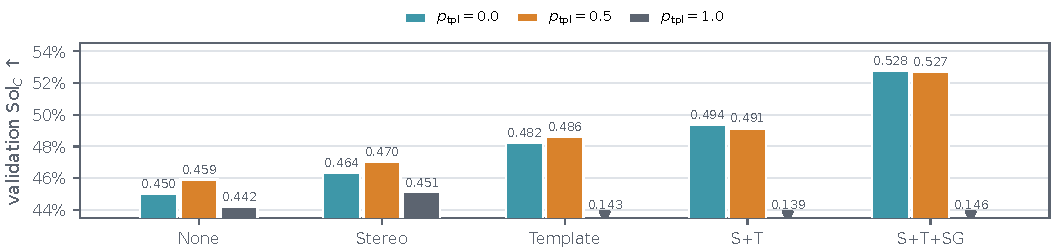
\includegraphics[width=\textwidth]{figures/generated/fig_conditioning_sweep.pdf}
  \caption{\textbf{Moderate template dropout is most robust across conditioning
    settings.} Validation $\mathrm{Sol}_C$ at epoch 300 using EDM--Heun with
    200 steps and 30 candidates per target. S, T, and SG denote stereochemistry,
    template coordinates, and space-group conditioning, respectively. Among
    models trained with $p_{\mathrm{tpl}}\in\{0,0.5,1\}$,
    $p_{\mathrm{tpl}}{=}0.5$ achieves the highest average performance across the
    five inference-time conditioning settings and is therefore selected.
    Template-conditioned results for $p_{\mathrm{tpl}}{=}1$ fall below the
    plotted range and are shown as downward triangles.}
  \label{fig:conditioning-sweep}
\end{figure}